\documentclass[a4paper,11pt]{article}
\usepackage[utf8]{inputenc}
\usepackage{geometry}
\usepackage{soul}
 \geometry{
 a4paper,
 total={170mm,257mm},
 left=25mm,
 right=25mm,
 top=18mm,
 bottom=19mm,
 }
 \usepackage{graphicx}
 \usepackage{titling}
 \usepackage{eurosym}
\usepackage{lipsum}  
\usepackage{cmbright}
\usepackage{listings}
\usepackage[spanish]{babel}
 
\usepackage{fancyhdr}
\fancypagestyle{plain}{%  the preset of fancyhdr 
    \fancyhf{} % clear all header and footer fields
   % \fancyfoot[R]{
\includegraphics[width=2cm]{UGR_LOGO.png}}
   % \fancyfoot[L]{\thedate}
    \fancyhead[L]{MUIT - Sistemas Electrónicos Integrados}
    \fancyhead[R]{\theauthor}
}



\begin{document}

\begin{titlepage}
 
 
\newlength{\centeroffset}
\setlength{\centeroffset}{-0.5\oddsidemargin}
\addtolength{\centeroffset}{0.5\evensidemargin}
\thispagestyle{empty}

\noindent\hspace*{\centeroffset}\begin{minipage}{\textwidth}

\centering

\includegraphics[width=0.9\textwidth]{imagenes/logo_ugr.jpg}\\[1.4cm]

\textsc{ \Large Proyecto de sistemas electrónicos integrados}\\[1cm]
% Upper part of the page
% 
% Title
{\LARGE \bfseries Diseño de un sistema de captación de señales satelitales NOAA con corrección de efecto Doppler\\
}
\noindent\rule[-1ex]{\textwidth}{3pt}\\[3.5ex]
{\large\bfseries Recepción y procesamiento de imágenes APT.}
\end{minipage}

\vspace{1cm}
\noindent\hspace*{\centeroffset}\begin{minipage}{\textwidth}
\centering

\textbf{Autores}\\ {Andrés Biedma Pérez\\Javier Lobato Martín\\Sergio Zapata Caparrós}\\[2.5ex]
\textbf{Director}\\
{Javier Díaz Alonso}\\[2cm]

\includegraphics[width=0.3\textwidth]{imagenes/etsiit_logo.png}\\[0.1cm]
\textsc{Escuela Técnica Superior de Ingenierías Informática y de Telecomunicación}\\
\textsc{---}\\
Granada, Enero de 2023
\end{minipage}
%\addtolength{\textwidth}{\centeroffset}
%\vspace{\stretch{2}}
\end{titlepage}






\section{Introducción}

\section{Distribución del proyecto}


\section{Hardware}

	\subsection{Antena}
	\subsection{RTL-SDR}

\section{Software}

	\subsection{Programa Gpredict}

	\subsection{Diagrama de flujo en GNU Radio}
	Con el propósito de procesar la señal recibida del RTL-SDR a tiempo real se ha creado un diagrama de bloques en GNU Radio. Los pasos a realizar en el procesamiento de la señal se han realizado teniendo en cuenta el estándar APT y son los siguientes:
	\begin{enumerate}
	\item Filtrado paso baja y decimado
	\item Demodulación FM
	\item Remuestreo a la frecuencia de audio
	\item Demodulación AM y construcción de la imagen
	\end{enumerate}
	
	\begin{figure}[hbtp]
 \centering
 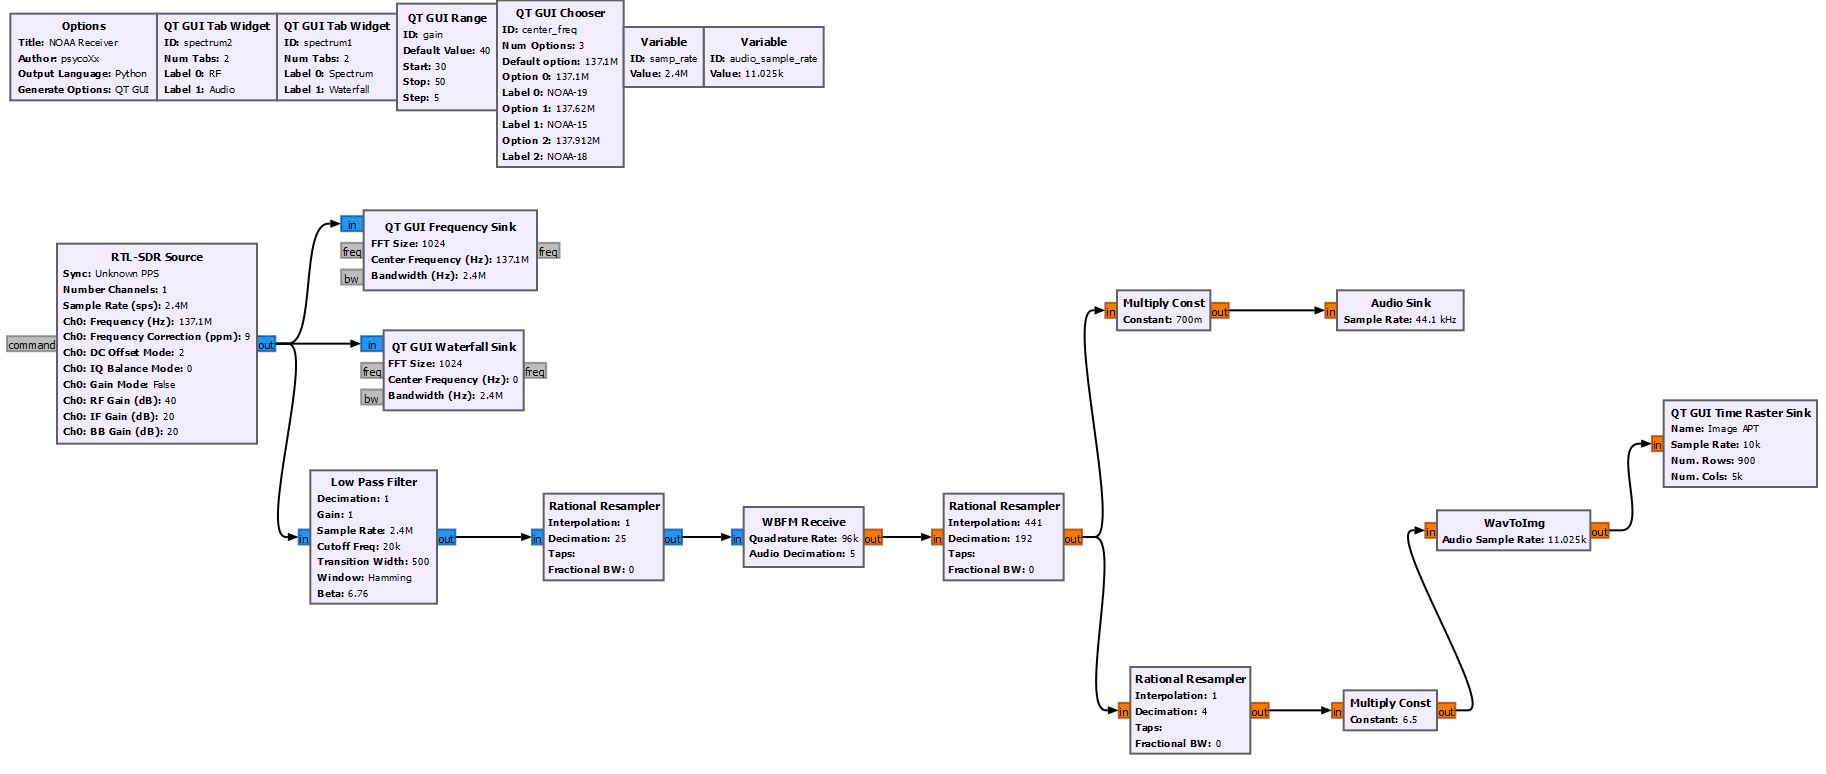
\includegraphics[width = 17cm]{imagenes/diagrama_flujo_completo.JPG}
 \caption{Diagrama de flujo}
 \label{diagrama_completo}
 \end{figure}
 
 En la \textit{Figura \ref{diagrama_completo}} se aprecia el diagrama de flujo completo. Después de obtener la señal de audio a la frecuencia de $11.025 kHz$, se llega a un bloque jerárquico llamado \textit{WavToImg} el cual realiza la correspondiente conversión de señal de audio a imagen APT. El interior de este bloque se muestra en la \textit{Figura \ref{wavtoimage}}.
 
 \begin{figure}[hbtp]
 \centering
 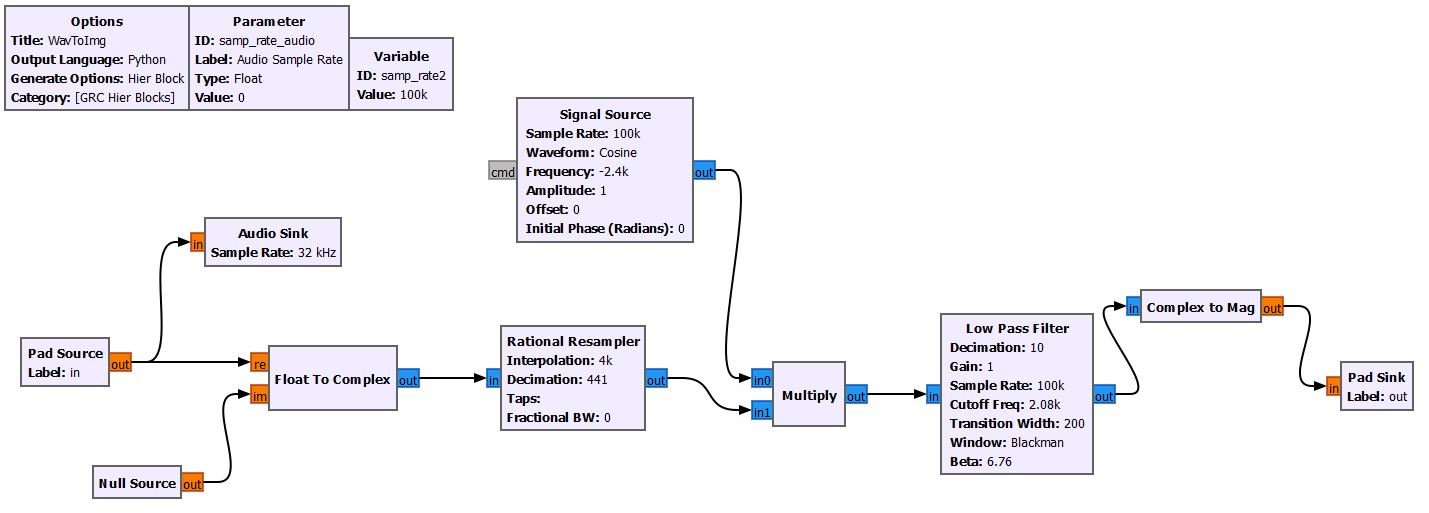
\includegraphics[width = 17cm]{imagenes/APT_hier.JPG}
 \caption{Bloque "WavToImg"}
 \label{wavtoimage}
 \end{figure}

El procedimiento se basa en una demodulación AM teniendo en cuenta que la información APT de interés se encuentra en una subportadora de $2.4 kHz$. 
	Según el estándar, se recomienda hacer un remuestreo a una frecuenciad e $100 kHz$ antes de hacer la demodulación. Para llevar la subportadora a banda base se ha utilizado un coseno a una frecuencia de $-2.4 kHz$ y se ha hecho un filtrado posterior.
	
La salida del bloque "WavtoImg" proporciona la señal APT demodulada y se muestra la imagen por pantalla a tiempo real.



	\subsection{Efecto Doppler}

\section{Resultados}

\section{Dificultades en la realización del proyecto}

\section{Conclusiones y líneas futuras}
 



\end{document}
